
%        File: WeeklyResearchReport_4_19_21.tex
%     Created: Mon Apr 19 08:00 AM 2021 E
% Last Change: Mon Apr 19 08:00 AM 2021 E
%
\documentclass[a4paper]{article}
\usepackage{mathtools}
\usepackage{verbatim}
\usepackage{graphicx}
\usepackage{tabularx}
\usepackage{pgfplots}
\usepackage{adjustbox}
\usepackage{booktabs}
\makeatletter
\let\latex@xfloat=\@xfloat
\def\@xfloat #1[#2]{%
    \latex@xfloat #1[#2]%
    \def\baselinestretch{1}
    \@normalsize\normalsize
    \normalsize
}
\makeatother
\usepackage{amsmath}
\usepackage{mathtools}
\usepackage{epigraph}
\usepackage{cancel}
\usepackage{xcolor}
\newcommand\Ccancel[2][black]{\renewcommand\CancelColor{\color{#1}}\cancel{#2}}
\usepackage{algorithm}
\usepackage{graphicx}
\usepackage[noend]{algpseudocode}
\usepackage{gnuplot-lua-tikz}
\usepackage[utf8]{inputenc}
\usepackage{pgfplots}
\usepackage{tabularx}
\DeclareUnicodeCharacter{2212}{−}
\usepgfplotslibrary{groupplots,dateplot}
\usetikzlibrary{patterns,shapes.arrows}
\pgfplotsset{compat=newest}
\begin{document}
\begin{titlepage}

    \title{
    Daily Research Report}

    \author{ Jeffrey Severino \\
        University of Toledo \\
        Toledo, OH  43606 \\
    email: jseveri@rockets.utoledo.edu}


    \maketitle

\end{titlepage}
\section{Current Research Direction}
The goal is to complete the validation for SWIRL by creating a range of test
cases.
\section{Research Performed}
The axial wavenumbers for a uniform flow case where $m = 2$ , $M = 0.3$ and 
$k = -1$ is presented. 
 \begin{figure}
     \centering
     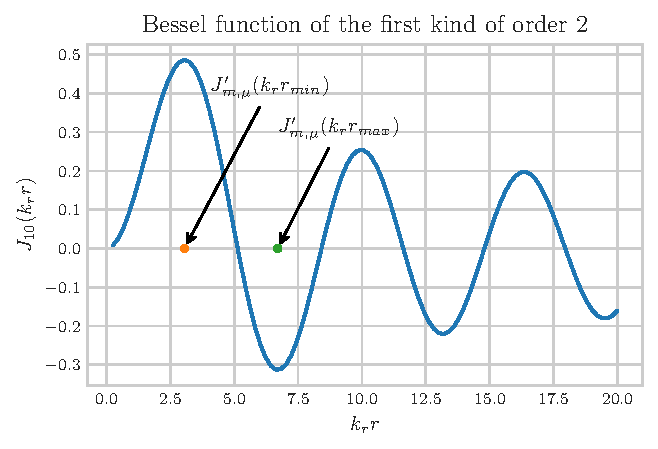
\includegraphics[width=\textwidth]{/home/jeff-severino/SWIRL/CodeRun/03-plotReport/tex-outputs/analytical_bessel_function.pdf}
     \caption{Bessel Function of the First Kind with the zero crossings of its
     derivative identified}
 \end{figure}

 \begin{figure}[h!]
     \centering
     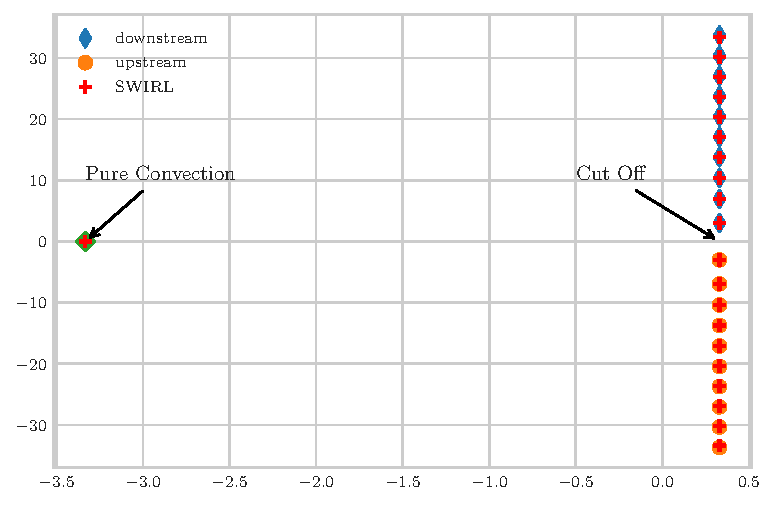
\includegraphics[width=\textwidth]{/home/jeff-severino/SWIRL/CodeRun/03-plotReport/tex-outputs/T1.pdf}
 \end{figure}

 The acoustic modes are along the cut off line (parallel to the imaginary axis)
 and the convective modes are to the left or right of the line. There were 
 mistakes in the AnalyticalDuctMode documentation and those were corrected
\section{Issues and concerns}
There was a realization (from yesturdays report) that the analytical solution for an annular duct is different
that for a cylindrical duct. That means that the expression provided may not 
be correct for the test cases in Kousen's work. I believe Amr's expression should be
used instead.
\section{Planned Research}
Try a different expression for an annular duct and see if there is better agreement.

\end{document}


